\chapter{Fundamentação Teórica}

Neste capítulo serão apresentadas as bases teóricas que permeiam o escopo do presente trabalho.
Partindo do entendimento sobre o conceito de arquitetura de software e como ela reflete nos
sistemas. Em seguida, abordando estilos de arquitetura de software pertinentes para o contexto
estudado. As seções estão dispostas em:

  \begin{enumerate}
    \item \textbf{Arquitetura de software:} definição do termo arquitetura dentro da área de
        software e suas características.
    \item \textbf{Sistemas monolíticos:} descrição, vantagens e desvantagens da arquitetura monolítica.
    \item \textbf{Microsserviços:} descrição, vantagens e desvantagens da arquitetura de
        microsserviços.
  \end{enumerate}

\section{Arquitetura de Software}

\begin{quotation}{Bass2015:SoftwareArchitetureInPratice}{transleted=true}
Software systems are constructed to satisfy organizations' business goals. The architecture is a bridge between those (often abstract) business goals and the final (concrete) resulting system. While the path from abstract goals to concrete systems can be complex, the good news is that software architecture can be designed, analyzed, documented, and implemented using know techniques that will support the achievement of these business and mission goals. The complexity can be tamed, made tractable.
\end{quotation}

Como retratado na citação acima, arquitetura de software representa a ponte entre os sistemas
construídos e os objetivos de cada organização. A publicação \textit{What is your definition of
software architecture?} do \textit{Software Engineering Institute} da \textit{Carnegie Mellon
University} \cite{SEI2017:WhatIsYourSoftwareArchitectureDefinition} apresenta uma variedade de diferentes
conceitos a respeito de arquitetura de software abordados pela bibliografia, exemplificando a
dificuldade existente em compreender o conceito de arquitetura dentro da área de \gls{TI}.

Segundo \citeonline{Vogel2011:SoftwareArchiteture} arquitetura é um aspecto implícito com o qual os desenvolvedores são confrontados
diariamente e que não pode ser ignorado ou eliminado, ainda que eles nem sempre tenham consciência
sobre a sua constante presença.

\citeonline{Bass2015:SoftwareArchitetureInPratice} traz a seguinte definição a respeito de
arquitetura de software:

\begin{quotation}{Bass2015:SoftwareArchitetureInPratice}{transleted=true}
The software architecture of a system is the set of structures needed to
reason about the system, which comprise software elements, relations
among them, and properties of both.
\end{quotation}

Com base nessa abordagem, os autores defendem que os sistemas de software são compostos por diversas
estruturas e elementos, por como essas estruturas se relacionam entre si e pelas propriedades que os
caracterizam. Assim, a arquitetura se torna uma abstração do sistema, destacando aspectos desejados
do mesmo e omitindo outros aspectos, com o intuito de minimizar a complexidade com a qual o compreendemos.

A \autoref{fig:ArchitectureDefinition} apresenta uma segunda visão abordada por
\citeonline{Richards2020:FundamentalsOfSoftwareArchitecture} a respeito de arquitetura.
Nessa abordagem eles defendem quatro dimensões as quais definem o que é arquitetura de software. A primeira
dimensão consiste nas estruturas: serviços, camadas e módulos são exemplos de conceitos abarcados
por esse ponto, todavia, para eles descrever a arquitetura por meio de estruturas não é suficiente para contemplar
todo o escopo acerca de arquitetura de software. Diante desta problemática, eles introduzem os
conceitos de características, decisão e princípios de design referentes a arquitetura. 

\begin{figure}[h]
  \centering
  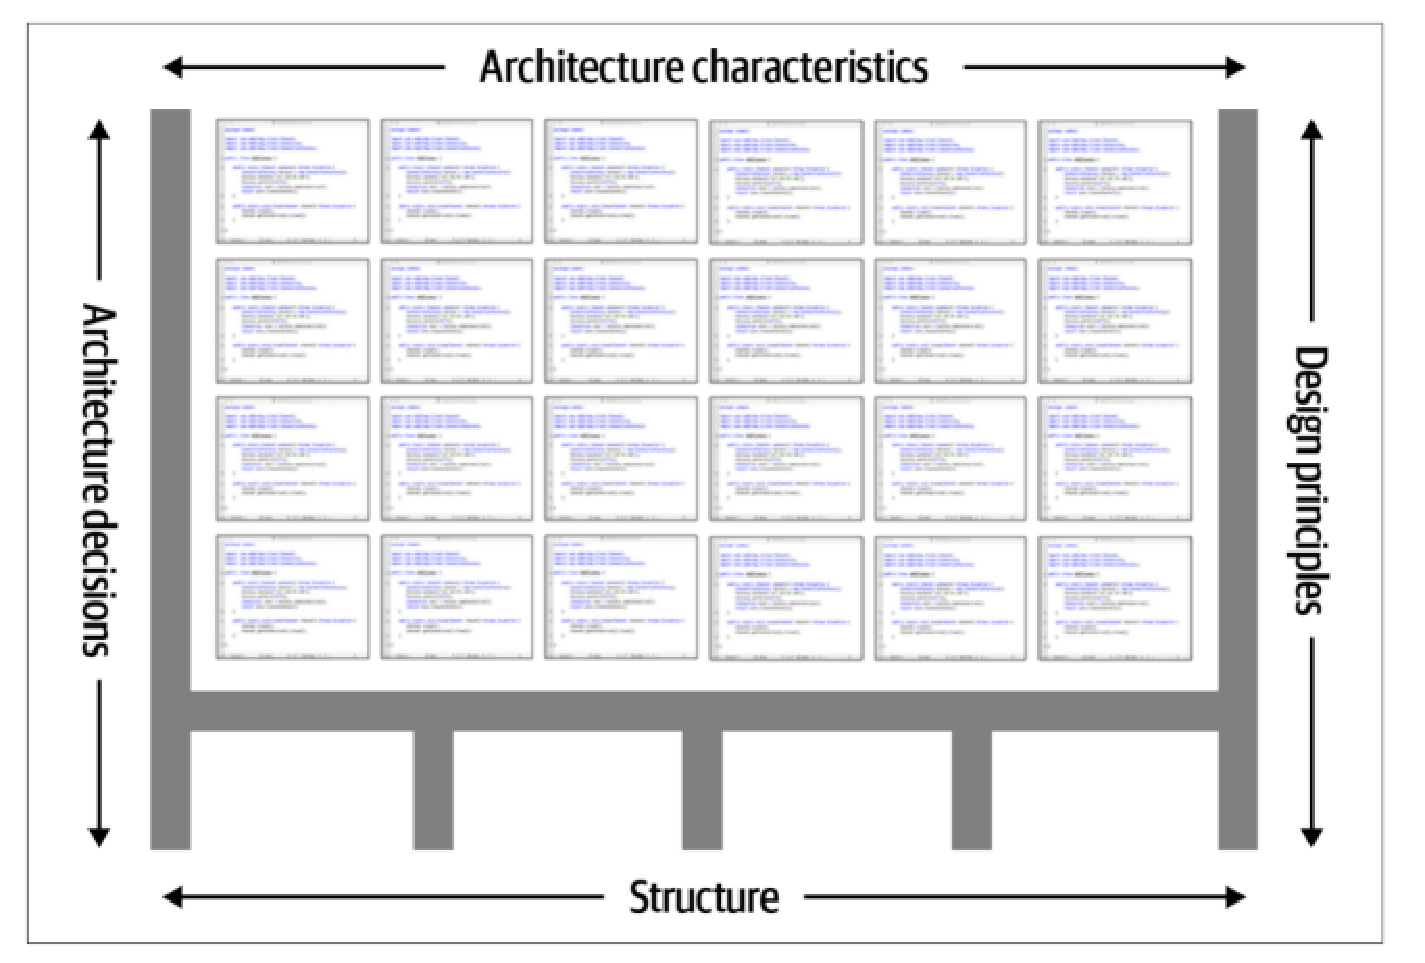
\includegraphics[keepaspectratio=true,scale=0.6]{figuras/richardsAndFord-architectureDefinition.eps}
  \caption{Elementos que compõem a arquitetura de um software\label{fig:ArchitectureDefinition} \source{Richards2020:FundamentalsOfSoftwareArchitecture}}
\end{figure}

As características da arquitetura, por sua vez, referem-se aos critérios de sucesso do sistema,
trazendo pontos como disponibilidade, confiabilidade, segurança, etc., os quais são anteriores e
independentes ao conhecimento acerca das funcionalidades que o software implementará.

O terceiro aspecto apresentado pelos autores consiste nas decisões de arquitetura responsáveis por definir
as regras sob as quais o sistema deve ser construído. Isto diz ao time de desenvolvimento o que ele
pode ou não fazer. A exemplo, em uma arquitetura \gls{MVC}\footnote{\textit{Model-View-Controller} (MVC)
consiste em um estilo arquitetural adotado por várias aplicações. A \textit{Model} representa a
camada de dados, a \textit{View} a camada de apresentação e a \textit{Controller} é a camada de
lógica \cite{mcgovern2004practical}.}, a \textit{View} é
impossibilitada de consumir dados da \textit{Model}, e cabe aos desenvolvedores garantir que isso
seja respeitado.

Por fim, a última dimensão refere-se aos princípios de design. Estes consistem em um guia pelo o qual
os desenvolvedores podem se orientar quando for necessário tomar alguma decisão. Diferentemente das
decisões de arquitetura que devem ser sempre seguidas afim de  garantir as características desejadas
para a arquitetura, os princípios trazem maior flexibilidade e autonomia para o desenvolvedor, podendo
este analisar o contexto do problema em mãos e decidir se seguir os princípios é a melhor abordagem
para a funcionalidade desenvolvida, ou se deve seguir por um caminho diferente o qual ele julgue que
os ganhos são maiores para a aplicação.

\subsection{Leis da Arquitetura de Software}

\begin{quotation}{Richards2020:FundamentalsOfSoftwareArchitecture}{transleted=true}
  \begin{description}
    \item [Tudo em arquitetura de software é um \textit{trade-off}.] Primeira Lei da Arquitetura de
        Software
    \item [\textit{Por que} é mais importantes do que \textit{como}.] Segunda Lei da Arquitetura de Software
  \end{description}\footnote{Texto original: \textit{Everything in software architecture is a trade-off. First Law
    of Software Architecture. Why is more important than how. Second Law of Software Architecture.}}
\end{quotation}

As leis acima foram apresentadas recentemente por \citeonline{Richards2020:FundamentalsOfSoftwareArchitecture}
no livro \textit{Fundamentals of Software Architecture: An Engineering Approach} e trazem consigo
perspectivas importantes para compreender o que é arquitetura de software dentro do dia a dia dos
engenheiros de software e como os mesmos devem lhe dar com ela.

A Primeira Lei da Arquitetura de Software descreve a realidade do arquiteto de
software, o qual precisa lidar constantemente com conflitos de escolha. O papel do arquiteto está
intrinsecamente ligado a análise da situação e a tomada de decisão sobre qual caminho seguir. Para
tal, é necessário que o mesmo esteja alinhado com uma série de fatores, como práticas de engenharia,
\textit{DevOps}\footnote{\textit{DevOps} é um movimento cultural que altera como indivíduos pensam
sobre o seu trabalho, dando suporte a processos que aceleram a entrega de valor pelas empresas ao
desenvolverem práticas sustentáveis de trabalho \cite{davis2016effective}.}, processos, negócio, etc
\cite{Richards2020:FundamentalsOfSoftwareArchitecture}.

A segunda lei traz uma perspectiva que por diversas vezes é ignorada, na qual tendemos a olhar para
a topologia dos sistemas, observando suas estruturas e como estas se relacionam, e não damos a devida
atenção ao porquê das decisões arquiteturais tomadas \cite{Richards2020:FundamentalsOfSoftwareArchitecture}.

Nesse sentindo, o ponto defendido pelos autores busca olhar o por quê certas decisões são
tomadas mediante os \textit{trade-offs} enfrentados.

\section{Sistemas monolíticos}

A visão inicial a respeito da Arquitetura Monolítica refere-se a um padrão de desenvolvimento
de software no qual um aplicativo é criado com uma única base de código, um único sistema de compilação,
um único binário executável e vários módulos para recursos técnicos ou de negócios. Seus componentes
trabalham compartilhando o mesmo espaço de memória e recursos formando uma unidade de
código coesa \cite{NatalliaSakovich}.

\citeonline{newman2019monolith} expande um pouco dessa visão, saindo da ideia de uma única base
de código coesa e adotando a perspectiva de uma única unidade de \textit{deploy}. Essa abordagem
permite a ele distinguir os seguintes tipos de monolíticos:

\begin{description}
    \item [Monolítico com um único processo] é o tipo mais comum de monolíticos e refere-se
        fundamentalmente a existência de um único processo executando toda a base de código. Vale
        ressaltar que dentro desta classificação exite ainda um subconjunto de monolíticos
        modulares nos quais têm se cada módulo trabalhando de forma independente um do outro, mas
        ainda com a necessidade de implantar uma única unidade de código.

    \item [Monolítico distribuído] são sistemas compostos por múltiplos serviços mas que precisam
        ser implantados juntos. Nas palavras de \citeonline{newman2019monolith}:

        \begin{quotation}{newman2019monolith}{transleted=true}
        Um monolítico distribuído pode muito bem atender a definição de uma \gls{SOA}, mas muitas vezes
        falha em cumprir as promessas do padrão.\footnote{Texto original: \textit{A distributed
        monolithic may well meet the definition of a service oriented-architecture, but all too
        often fails to deliver on the promises of SOA.}}
        \end{quotation}
    \item [Sistemas caixa preta de terceiros] também são abordados por \citeonline{newman2019monolith}
        como sendo monolíticos, uma vez que não é possível decompor os esforços referente a uma
        migração.
\end{description}

% Contudo, a longo prazo começam a surgir dificuldades para manter essa
% arquitetura, entre elas estão:
%
%   \begin{enumerate}
%     \item Dificuldade em entender e alterar o código que ao longo do tempo se torna
%     muito extenso e coeso;
%     \item Limitação na agilidade de atualização do software, uma vez que para cada
%     pequena alteração é necessário reimplantar o código por completo;
%     \item Necessita de muito esforço para adotar uma nova tecnologia, sendo
%     necessário adaptar todo o código da aplicação para a nova ferramenta;
%     \item O sistema perde a confiabilidade pois a medida que cresce um \textit{bug}
%     em uma única parte do código pode interromper todo o software já que todos os
%     componentes estão conectados.
%   \end{enumerate}

\section{Microsserviços}

Segundo \citeonline{Newman2015}, microsserviços são pequenos serviços autônomos que
trabalham juntos. O objetivo desses serviços é tornar o código coeso e focado em
resolver as regras de negócio dentro de um limite específico. As vantagens de adotar
essa arquitetura consistem em:

\begin{enumerate}
    \item{Uso de tecnologias heterogêneas;}
    \item{Maior resiliência do sistema;}
    \item{Facilidade em escalar pequenas partes do sistema, ao invés do sistema por
    completo;}
    \item{Facilidade e maior estabilidade no processo de \textit{deploy};}
    \item{Maior produtividade da equipe, uma vez que se passa a adotar equipes
    menores com bases de código menores;}
    \item{Reusabilidade dos serviços;}
    \item{Otimização da substituibilidade: organizações de médio e grande porte costumam
    possuir sistemas legados, com uma base de código enorme funcionando com tecnologias
    antigas tanto de software quanto de hardware. A substituição desses códigos é um
    processo custoso e arriscado. Com serviços pequenos realizar essa substituição
    se torna um processo mais fácil de gerenciar.}
\end{enumerate}

Para o desenvolvimento de microsserviços é necessário pensar sobre o que deve ser
exposto e o que deve ser ocultado. Se houver muito compartilhamento os serviços de
consumo se acoplam às nossas representações internas, diminuindo a nossa autonomia
e consequentemente a nossa capacidade de realizar alterações \cite{Newman2015}.

\section{Perspectivas a respeito de cada estilo arquitetural}

Esta seção visa aprofundar no entendimento sobre as vantagens e desafios encontrados na adoção
de cada um dos estilos arquiteturais abordados nesse trabalho. Para tal, será explorado as seguintes
perspectivas com o intuito de compreender como a escolha da arquitetura impacta ou é impactada pelas
mesmas:

\begin{enumerate}
    \item Problemática a ser resolvida;
    \item Recursos necessários
    \item Características arquiteturais;
    \item Manutenibilidade;
    \item Evolucionabilidade.
\end{enumerate}

\subsection{Problemática a ser resolvida}
\label{Perpectivas:Problematica}

Ao iniciar um projeto é comum se ter um baixo domínio sobre o problema a ser resolvido. A exemplo,
as denominadas \textit{startups} estão continuamente surgindo no mercado com o intuito de descobrir
e validar suas ideias. Contextos como este trazem as empresas a necessidade de realizar constantes
alterações de forma extremamente rápida no sistema visando atingir um curto ciclo de
\textit{feedback}.

\citeonline{MartinFowler:MonolithFirst} defende que construir uma versão simplista do seu software é
a melhor forma de descobrir o sistema e validar se ele é realmente útil para os seus usuários.
Assim, ele sugere a estratégia "monolítico primeiro", uma vez que a arquitetura monolítica permite
um desenvolvimento fácil por ser de conhecimento da maioria dos desenvolvedores de software e
apresentar baixa complexidade para a execução de tarefas como \textit{deploy}, confecção de testes
e compartilhamento do código.

\citeonline{MartinFowler:MonolithFirst} e \citeonline{Newman:Greenfield} fortalecem essa visão apontando
que conhecer os limites do seu software é de extrema importância antes de iniciar uma arquitetura de
microsserviços. De forma que os custos e impactos de errar os limites de cada serviço nessa arquitetura
tendem a ser muito maiores do que em um software monolítico mal projetado por não conhecer muito bem o
domínio do problema. 

Um outro ponto a ser considerado na problemática da aplicação refere-se ao tamanho que essa
aplicação terá. \citeonline{Richards2020:FundamentalsOfSoftwareArchitecture} apontam que a arquitetura
monolítica é uma arquitetura de menor custo portanto costuma ser uma boa escolha para sistemas
pequenos.

\subsection{Recursos necessários}

\subsubsection{Recursos financeiros}

De acordo com \cite{Richards2020:FundamentalsOfSoftwareArchitecture}, a simplicidade da arquitetura
monolítica reflete em seu baixo custo de desenvolvimento e manutenção. Diferentemente, de uma arquitetura
de microsserviços que exige uma série de fatores: monitoramento, replicação, expertise sobre as
ferramentas, etc., fazendo com o que o custo para desenvolver e manter tal arquitetura seja elevado.
Mediante essa visão, os autores indicam o uso desse modelo para empresas de grande porte,
enquanto que empresas pequenas tendem a lhe dar melhor com monolíticos.

\subsubsection{Recursos humanos}

Na seção \autoref{Perpectivas:Problematica}, nós enfatizamos a importância de conhecer os limites da
sua aplicação antes de optar por uma arquitetura de microsserviços. Isso nos leva a uma outra necessidade desse
estilo arquitetural, referente a relevância de possuir alguém na equipe que detenha esse conhecimento
aprofundado acerca do negócio e da problemática abordada. No texto \textit{Microservices For
Greenfield?}, \citeonline{Newman:Greenfield} relata um projeto no qual eles estavam reimplementando
um sistema que já existia há muitos anos, mas com uma equipe relativamente nova, ou seja, apesar do
domínio de negócio ter sido explorado por um bom tempo, eles não possuíam a expertise necessária
para a construção da aplicação de forma distribuída.

Nesse contexto, \citeonline{Newman:Greenfield} indica a adoção de uma arquitetura monolítica como uma
melhor opção uma vez que, como citado na \autoref{Perpectivas:Problematica}, este estilo arquitetural
é indicado para contextos nos quais não se possui domínio e, para completar, apresenta a vantagem de ser uma
arquitetura familiar para boa parte dos desenvolvedores
\cite{Richards2020:FundamentalsOfSoftwareArchitecture}, dessa forma, ele se diferencia de uma
arquitetura de microsserviços por não precisar de um especialista sobre a tecnologia e sobre o contexto.


\subsubsection{Esforço e tempo inicial}

O tempo de lançamento no mercado costuma ser um fator prioritário para diversas empresas, em geral,
elas desejam lançar o produto no menor tempo possível, seja para validar a ideia, como
vimos na \autoref{Perpectivas:Problematica}, ou por uma questão estratégica de mercado.

Nesse sentido, \citeonline{MartinFowler:MicroservicePremium} aponta que a arquitetura de
microsserviços consegue te entregar uma séries de recompensas (escalabilidade, tolerância a falhas,
etc.) contudo, essas recompensas vêem acompanhada do alto custo que é inerente dos sistemas distribuídos.
Esse modelo arquitetural necessita de \textit{deploy} automatizado, monitoramento, lidar com
eventuais inconsistências dos dados e outros fatores que acabam contribuindo para aumentar o tempo e o esforço
inicial necessário para lançar um produto no mercado. Nas palavras de
\citeonline{Richards2020:FundamentalsOfSoftwareArchitecture}:

\begin{quotation}{Richards2020:FundamentalsOfSoftwareArchitecture}{transleted=true}
    Microsserviços não poderiam existir sem a revolução \textit{DevOps} e a implacável marcha em direção à
    automação de questões operacionais.\footnote{Texto original: \textit{Microservices couldn't exist
    without the DevOps revolution and the relentless march toward automating operational concerns.}}
\end{quotation}

Por outro lado, a simplicidade da arquitetura monolítica permite que funcionalidades cheguem muito
mais rápido no mercado, uma vez que nesse modelo não há tais necessidades e processos como
\textit{deploy} podem ser realizados de maneira operacional. Contudo, vale ressaltar que essa alta
produtividade inicial tende a decrescer com o tempo, a medida que o monolítico vai ganhando mais
funcionalidades e, consequentemente, aumentando a sua complexidade.

\subsection{Características arquiteturais}

\susubsection{Escalabilidade}
\susubsection{Volume de dados}
\susubsectionT{Tolerância a falhas}
\susubsectionT{Confiabilidade}
\susubsectionT{Disponibilidade}
\susubsectionT{Performance}

% \iffalse
%
% Neste capítulo será apresentado as bases teóricas que permeiam o escopo
% do presente trabalho. Partindo do entendimento sobre o contexto de
% \textit{startups} até as questões relacionadas a escalabilidade de softwares.
%
%   \begin{enumerate}
%     \item \textbf{\textit{Startups}:} contexto, organização e propósitos de uma 
%       \textit{startup};
%     \item \textbf{Desenvolvimento de Software:} abordagem sobre boas práticas
%     de desenvolvimento de software e como estas estão sendo abordadas no contexto
%     de \textit{startups};
%     \item \textbf{Escalabilidade de Software:} definição de Escalabilidade e 
%       possíveis formas de aplicação.
%   \end{enumerate}
%
% \section{\textit{Startups}}
%
% No livro \textit{A Revolução das Startups} de \citeonline{ARevolucaoDasStartups},
% o autor descreve uma Geração Y, nascida entre 1980 e 2000, detentora de um
% espírito jovem em busca de ser feliz fazendo algo que seja realmente
% impactante para a sociedade. Diferente das gerações passadas, a Geração Y
% possui em suas mãos a Internet e o conhecimento para utilizar esta
% ferramenta em todo o seu potencial.
%
% Essa geração leva a sociedade a um contexto no qual as pessoas estão sempre
% se questionando se existe outra forma de fazer, se podemos fazer melhor e
% se somos capazes de resolver algum problema \cite{ARevolucaoDasStartups}.
% A partir dessas indagações nascem \textit{startups} revoluniciárias, como
% o Waze\footnote{Empresa que conecta motoristas visando melhorar o tráfego
% dentro das cidades. Saiba mais em: \url{https://www.waze.com}}, lançado em
% 2009 com a proposta de mudar a forma das pessoas se locomoverem, deixando 
% de lado a maneira tradicional de se usarem mapas e fazendo com que as 
% pessoas interajam e contribuam para o próprio mapeamento
% \cite{NepomucenoSucessoDoWaze}.
%
% \subsection{O que é uma \textit{Startup}?}
% \label{sec:OQueEUmaStartup}
%
% \begin{quotation}{SteveBlankFirstPrinciples}{transleted=true}
% Uma \textit{startup} é uma organização formada para buscar um modelo de 
% negócios repetível e escalável.\footnote{Texto original: \textit{A startup is an
% organization formed to search for a repeatable and scalable business model.}}
% \end{quotation}
%
% A definição apresentada por Steve Blank traz características
% fundamentais para entender o conceito de uma \textit{startup}. Começando
% pela organização que representa um grupo de pessoas alinhadas em prol
% de um mesmo objetivo. Esse grupo de pessoas juntamente com seus ideais
% são a essência de uma \textit{startup}, afinal, são elas que fazem
% o negócio fluir somando as habilidades individuais de cada um
% \cite{ARevolucaoDasStartups}.
%
% O modelo de negócio é a descrição de como a empresa cria, entrega e captura
% valor, exibindo todos os fluxos entre as diferentes partes da empresa,
% como o produto é distribuído para os clientes, como o dinheiro retorna, a
% estruturas de custos e a interação com outras empresas parceiras. Uma
% \textit{startup} consiste essencialmente em uma organização criada para
% procurar um modelo de negócios, iniciando com uma visão sobre o produto e
% uma série de hipóteses sobre o modelo de negócios
% \cite{SteveBlankFirstPrinciples}.
%
% Segundo \citeonline{ARevolucaoDasStartups}, ser repetível significa que 
% a ideia deve ser facilmente replicável em outras regiões, países ou até
% mesmo outros setores, visando diversificar os ganhos. Ou seja, quanto mais
% pessoas utilizam o serviço, melhor para as \textit{startups}.
%
% Atingir o objetivo de ser repetível carrega junto a missão de ser também
% escalável. Afinal, reproduzir o modelo de negócio em outras regiões e países
% também envolve a capacidade da empresa de crescer, preferencialmente de uma
% forma saudável. Para tal é necessário que os serviços sejam prestados sem
% demandar recursos na mesma proporção que o seu crescimento, usando somente 
% uma estrutura básica comum a todos \cite{CassioSpina}.
%
% No livro \textit{A Startup Exuta}, \citeonline{StartupEnxuta} traz outra
% definição de \textit{startup} a qual diz que \begin{quote}Startup é uma instituição
% humana projetada para criar novos produtos e serviços sob condições de extrema
% incerteza\end{quote}. Um contexto no qual toda aprendizagem é válida e deve ser
% reutilizada em um ciclo constante de coleta de \textit{feedbacks} dos clientes.
%
% Essa segunda definição, adiciona uma nova característica ao conceito de
% \textit{startup} que é o ambiente extremamente incerto no qual essas empresas
% estão inseridas. Com base em  \apudonline{Rueda}{GardelinRausp}, esta incerteza
% ambiental é perceptível em uma empresa quando há dúvidas, por parte dos gerentes,
% quanto a uma série de fatores, entre eles: a viabilidade de futuras tecnologias,
% as expectativas de mudanças de consumo e preferências sociais para os produtos
% e serviços e possíveis mudanças na legislação.
%
% \subsection{Fases de uma Startup}
%
% De acordo com \citeonline{Blank2013} no seu livro \textit{The four steps to the Epiphany},
% o modelo de desenvolvimento que melhor se adapta ao contexto de uma \textit{startup}
% é o Modelo de Desenvolvimento do Cliente, apresentado na \autoref{fig:FourStepsToEpiphany}.
% \citeonline{Blank2013} defende que este modelo não é um substituto para o Modelo de
% desenvolvimento do Produto tradicionalmente adotado nas grandes empresas, mas sim
% um complemento que se concentra na compreensão dos problemas e nas necessidades
% do cliente. Este modelo é caracterizado por quatro fases, sendo elas:
%
% \begin{figure}[h]
%   \centering
%   \includegraphics[keepaspectratio=true,scale=0.6]{figuras/epiphany.eps}
%   \caption{Modelo de desenvolvimento do Cliente\label{fig:FourStepsToEpiphany} \source{Blank2013}}
% \end{figure}
%
% \begin{description}
%     \item[Passo 1: Descoberta do cliente] O objetivo desta etapa é descobrir quem
%     são os clientes para o produto proposto e se o problema que está sendo solucionado
%     é de fato importante para eles. Nesse sentindo, a primeira ideia e requisitos
%     sobre o produto originam-se na verdade a partir dos fundadores da \textit{startup},
%     e é papel do Time de Desenvolvimento do Cliente verificar se existe clientes
%     e um mercado para tal visão.
%     \item[Passo 2: Validação do cliente] Esta etapa tem por objetivo montar um
%     roteiro de vendas repetível para as equipes de marketing e vendas seguirem adiante.
%     O propósito desse roteiro é guiar a equipe com base em experiências de campo nas
%     quais a venda foi bem sucedida para os primeiros clientes. Esta validação mostra
%     que foi encontrado um conjunto de clientes interessados e um mercado que reage
%     positivamente ao produto.
%     \item[Passo 3: Criação do cliente] Com base no sucesso das vendas iniciais, esta
%     etapa dedicasse a criar uma demanda no usuário final. Nesta etapa o produto já foi
%     validado e agora os investimentos em marketing podem ser altos, permitindo que a
%     empresa controle sua taxa de queima de caixa e proteja seus ativos.
%     \item[Passo 4: Construção da Empresa] É a etapa na qual a empresa faz a transição da
%     sua equipe de Desenvolvimento do Cliente, orientada para aprendizado e descoberta,
%     para departamentos formais de vendas, marketing, etc. Esses departamentos, por sua
%     vez, devem se concentrar em explorar o sucesso inicial da \textit{startup} no mercado.
% \end{description}
%
%
% \section{Desenvolvimento de Software}
%
% Segundo \citeonline{Despa2014} o processo de construção de um software consiste
% em vários estágios distintos, os quais são caracterizados por suas entregas em um
% período de tempo específico. Podemos classificar esses estágios nas seguintes
% atividades:
%
% \begin{description}
%     \item[Pesquisa]{é o estágio destinado a formulação dos requisitos, na qual os
%     envolvidos trocam informações a respeito do sistema que está sendo proposto,
%     definem metas que devem ser alcançadas e buscam características sobre o mercado,
%     o comportamento do usuário e soluções técnicas;}
%     \item[Planejamento]{é o estágio destinado a definição dos fluxos que a aplicação
%     terá que executar, com base nesses fluxos definisse também as tecnologias que
%     serão adotadas, como será organizado o banco de dados e a metodologia que será
%     aplicada durante o processo de construção;}
%     \item[Design]{é o estágio no qual a interface da aplicação é definida com base
%     no seu respectivo contexto. Esta etapa permite uma validação prévia com o cliente,
%     na qual costumam surgir novos requisitos e mudanças no sistema. Em geral, é possível
%     realizar essa etapa em paralelo a programação;}
%     \item[Desenvolvimento]{é a etapa na qual o software é de fato construído. Inicia-se
%     com a configuração do ambiente de desenvolvimento, o qual deve estar integrado com o
%     ambiente de teste. Nesta fase os desenvolvedores devem estar preocupados em não
%     inserir erros no código e deixar comentários que facilitem a manutenção depois;}
%     \item[Teste]{é o estágio destinado a identificação de erros tanto de implementação
%     quanto de design. Nessa etapa deve ser verificado se o software está de acordo com
%     os requisitos planejados, se não está sujeito a falhas de segurança e se existe
%     algum problema de usabilidade;}
%     \item[Implantação]{é o estágio no qual são realizadas todas as configurações e testes
%     necessários para disponibilizar a aplicação em um ambiente ativo para o usuário final.
%     Nesta fase, o sistema deve ser integrado com aplicativos de terceiros, caso seja
%     necessário, e configurado rotinas de backup;}
%     \item[Manutenção]{é o estágio subsequente a parte de implantação, e refere-se a etapa
%     na qual são identificados novos erros que possam ter passado despercebidos, adicionadas
%     novas funcionalidades e realizado o monitoramento do \textit{log} para a identificação
%     de erros e o monitoramento do tráfego, com o intuito de prever possíveis problemas de
%     de desempenho que a aplicação possa vir a sofrer.}
% \end{description}
%
% Os estágios mencionados acima são geralmente aceitos pela comunidade de software
% como os pilares do desenvolvimento de software. Estando, em sua maioria, presentes
% nas mais variadas metodologias de desenvolvimento, mesmo que com nomenclaturas
% diferentes \cite{Despa2014}.
%
% \subsection{Manifesto Ágil}
%
% O Manifesto Ágil é um conjunto de valores que visam auxiliar a descobrir como
% fazer as coisas certas dentro do seu contexto de projeto. Uma das características
% que destacam o Agile em relação a outras abordagens de desenvolvimento de software
% é foco nas pessoas que realizam o trabalho e como elas trabalham juntas. Abaixo
% segue os quatros valores declarados por \citeonline{AgileManifesto} no Manifesto Ágil:
%
% \begin{enumerate}
%     \item Indivíduos e interações mais que processos e ferramentas;
%     \item Software em funcionamento mais que documentação abrangente;
%     \item Colaboração com o cliente mais que negociação de contrato;
%     \item Responder a mudanças mais que seguir um plano.
% \end{enumerate}
%
% \subsection{Os 12 princípios do software ágil}
%
% Junto com os valores expressos no Manifesto Ágil, o desenvolvimento ágil de software
% é guiado pelos doze princípios apresentados a seguir:
%
% \begin{enumerate}
%     \item Nossa maior prioridade é satisfazer o cliente, através da entrega adiantada
%     e contínua de software de valor;
%     \item Aceitar mudanças de requisitos, mesmo no fim do desenvolvimento. Processos
%     ágeis se adequam a mudanças, para que o cliente possa tirar vantagens competitivas;
%     \item Entregar software funcionando com frequência, na escala de semanas até meses,
%     com preferência aos períodos mais curtos;
%     \item Pessoas relacionadas à negócios e desenvolvedores devem trabalhar em conjunto
%     e diariamente, durante todo o curso do projeto;
%     \item Construir projetos ao redor de indivíduos motivados. Dando a eles o ambiente e
%     suporte necessário, e confiar que farão seu trabalho;
%     \item O Método mais eficiente e eficaz de transmitir informações para, e por dentro
%     de um time de desenvolvimento, é através de uma conversa cara a cara;
%     \item Software funcional é a medida primária de progresso;
%     \item Processos ágeis promovem um ambiente sustentável. Os patrocinadores,
%     desenvolvedores e usuários, devem ser capazes de manter indefinidamente, passos
%     constantes;
%     \item Contínua atenção à excelência técnica e bom design, aumenta a agilidade;
%     \item Simplicidade: a arte de maximizar a quantidade de trabalho que não precisou ser
%     feito;
%     \item As melhores arquiteturas, requisitos e designs emergem de times auto-organizáveis;
%     \item Em intervalos regulares, o time reflete em como ficar mais efetivo, então, se
%     ajustam e otimizam seu comportamento de acordo.
% \end{enumerate}
%
% \subsection{Scrum}
%
% O Scrum pertence a família dos métodos ágeis e é uma metodologia de desenvolvimento
% de software iterativa e incremental baseada em \textit{timboxes} e voltada para o
% gerenciamento do projeto. Esta metodologia parte da premissa de que o desenvolvimento
% de software é muito complexo e imprevisível para ser planejado exatamente com
% antecedência. Neste caso, deve ser aplicado o controle empírico do processo afim de
% garantir transparência, inspeção e adaptação \cite{Mahnic2005}. Para tal, essa
% metodologia utiliza de papéis, eventos, artefatos e regras que os unem. A seguir,
% serão explicados cada um desses tópicos individualmente de acordo com as informações
% dispostas em \textit{The Scrum Guide} escrito por \citeonline{ScrumGuide}.
%
% \subsubsection{Papéis}
%
% \begin{description}
%     \item[\textit{Product Owner}] responsável por representar os interesses de
%     todos os envolvidos no projeto e em seu sistema resultante. Deve manter o
%     \textit{Product backlog} do projeto priorizado conforme as necessidades do cliente;
%     \item[Time de desenvolvimento] é uma equipe autogerenciada, auto-organizada e
%     multifuncional, responsável por implementar o \textit{Product backlog}. Os
%     membros da equipe são coletivamente responsáveis pelo sucesso de cada iteração
%     e do projeto como um todo;
%     \item[Scrum master] é o responsável por garantir a execução do processo Scrum.
%     Deve ensinar as práticas do Scrum aos envolvidos e incentivá-los a seguir essas
%     práticas afim de que a metodologia tenha sucesso na organização.
% \end{description}
%
% \subsubsection{Artefatos}
%
% Os artefatos do Scrum são produzidos com o objetivo de fornecer transparência e
% permitir inspeção e adaptação, visando maximizar a transparência das informações
% principais com o intuito de que toda a equipe tenha o mesmo entendimento a respeito
% do artefato.
%
% \begin{description}
%     \item[\textit{Product Backlog}] é uma lista ordenada com todas as funcionalidades
%     que se sabe que o produto deve contemplar. Esta lista nunca está completa e é
%     evoluída ao longo da execução do projeto com a finalidade de atender as necessidades
%     do cliente;
%     \item[\textit{Sprint Backlog}] é conjunto de itens oriundos do \textit{product backlog},
%     com o propósito de serem finalizados durante a execução da respectiva \textit{sprint};
%     \item[\textit{Incremento}] é a soma de todos os itens do \textit{product backlog}
%     entregues durante a \textit{sprint} e o valor dos incrementos de todas as \textit{sprints}
%     anteriores.
% \end{description}
%
% \subsubsection{Eventos}
%
% O objetivo dos eventos no Scrum é criar uma regularidade e minimizar a necessidade
% de reuniões durante o projeto. Cada evento tem um tempo determinado para acontecer,
% não podendo ultrapassar esse limite visando evitar desperdício de tempo durante o
% processo. Tais eventos são apresentados adiante:
%
% \begin{description}
%     \item[Sprint] é o \textit{timebox} principal do Scrum com duração de 1 mês ou
%     menos e o objetivo de criar um produto utilizável e potencialmente liberável.
%     Durante a \textit{sprint} são incluídos os outros eventos apresentados adiante;
%     \item[Sprint Planning] evento no qual o Time de Desenvolvimento, colaborativamente,
%     planeja o que será realizado durante a \textit{sprint} que se inicia. São
%     levantados aspectos sobre quais atividades do \textit{backlog} podem ser entregues
%     ao final da iteração e como será o trabalho necessário para alcançá-las;
%     \item[Daily] são reuniões diárias de no máximo 15 minutos. O objetivo destas
%     reuniões é verificar o andamento da \textit{sprint} e planejar o que será executado
%     nas próximas 24 horas. Dessa forma visa-se acompanhar e otimizar o andamento da
%     \textit{sprint};
%     \item[Sprint Review] realizado ao final da \textit{sprint} com o intuito de
%     inspecionar e adaptar o \textit{product backlog} com base no que foi entregue;
%     \item[Sprint Retrospective] realizado antes do próximo \textit{sprint planning}, é
%     uma reunião para a equipe se auto inspecionar e planejar melhorias para a próxima
%     \textit{sprint}.
% \end{description}
%
% A \autoref{fig:ScrumFramework} visa ilustrar o ciclo de vida do processo Scrum.
%
%     \begin{figure}[h]
%       \centering
%       \includegraphics[keepaspectratio=true,scale=0.4]{figuras/scrumFramework.eps}
%       \caption{Scrum Framework\label{fig:ScrumFramework} \source{WhatIsScrum}}
%     \end{figure}
%
% \subsection{Extreme Programming}
%
% A metodologia \gls{XP} é um processo ágil bastante popular que enfatiza a satisfação
% do cliente incentivando os desenvolvedores a responder com confiança as mudanças
% nos requisitos, ainda que no final do ciclo de vida do projeto. Ela divide o processo
% convencional de desenvolvimento de software em blocos menores e mais gerenciáveis visando
% minimizar posteriores custos de alteração \cite{Wells2000,Despa2014}. Esta metodologia é
% baseada nos seguintes cinco princípios:
%
% \begin{description}
%     \item[Simplicidade:] fazer somente o que é necessário e nada a mais que isso. Assim,
%     o valor entregue será maximizado e o projeto poderá ser mantido a longo prazo por
%     custos razoáveis;
%     \item[Comunicação:] todos fazem parte da equipe e devem se comunicar diariamente
%     sobre todas as áreas, desde requisitos a código, para que todos possam juntos
%     construir a melhor solução;
%     \item[Feedback:] o software deve ser demonstrado cedo e por muitas vezes, sendo
%     importante ouvir atentamente as observações e realizar as alterações necessárias.
%     O processo da equipe deve ser adaptado as necessidades do projeto, e não o contrário;
%     \item[Respeito:] todos dão e sentem o respeito que merecem como um membro valioso
%     da equipe. Toda contribuição é bem vinda e tem igual valor, independente se ela vem
%     do cliente, da gerência ou da equipe de desenvolvimento;
%     \item[Coragem:] deve-se sempre dizer a verdade sobre o progresso e as estimativas e
%     não ter medo de se adaptar as mudanças sempre que elas ocorrerem.
% \end{description}
%
% Nos sub tópicos adiante, serão apresentadas as regras que guiam a metodologia \gls{XP}
% em cada área do processo de desenvolvimento de acordo com \citeonline{Wells2000}.
%
% \subsubsection{Planejamento}
% \begin{description}
%     \item[Histórias de usuário devem ser escritas.] Histórias de usuário são frases escritas
%     pelo próprio cliente, sem nenhum linguajar técnico, que visam descrever coisas que o
%     sistema deve fazer. Muitas vezes são utilizadas no lugar de um grande documento de
%     requisitos e servem para criar estimativas quanto ao tempo durante a reunião de
%     planejamento;
%     \item[O planejamento do lançamento cria a programação de lançamento.] Deve ser realizada
%     uma reunião para traçar um plano de lançamento que estabeleça o projeto geral. Neste
%     planejamento são tomadas tanto decisões técnicas quanto decisões de negócios afim de
%     definir uma agenda com a qual todos os envolvidos podem se comprometer;
%     \item[Faça lançamentos pequenos e frequentes.] A equipe de desenvolvimento deve
%     liberar versões iterativas do sistema frenquentemente, pelo menos a cada duas semanas.
%     Assim no final de cada de iteração você terá testado e demonstrado a funcionalidade
%     para o cliente
%     \item[O projeto é dividido em iterações.] O cronograma deve ser dividido
%     em várias iterações de 1 a 3 semanas com o intuito de realizar constantemente pequenas
%     entregas;
%     \item[O planejamento da iteração inicia cada iteração.] Cada iteração deve iniciar com
%     o seu planejamento, no qual as histórias de usuários são selecionadas para serem
%     implementadas de acordo com a prioridade definida pelo cliente.
% \end{description}
%
% \subsubsection{Gerenciamento}
% \begin{description}
%     \item[Dê ao time um espaço de trabalho aberto e dedicado.] A comunicação é um
%     fator muito importante dentro do \acrlong{XP}. Aproximar a equipe fisicamente e
%     remover barreiras físicas entre eles incentiva-os a trabalhar colaborativamente
%     como um conjunto no qual todos tem igual valor e contribuições;
%     \item[Defina um ritmo sustentável.] O objetivo do \gls{XP} é conseguir um software
%     mais completo, testado, integrado e pronto para produção a cada iteração. Software
%     incompleto ou com erros representa uma quantidade desconhecida de esforços futuros
%     que não podem ser mensurados. Nessa perspectiva, a metodologia prega que se as
%     histórias planejadas para a iteração não puderem ser concluídas, o ideal é fazer
%     um novo planejamento da iteração visando definir o que será entregue até o final.
%     Mesmo que falte somente um dia para terminar a iteração, o melhor é focar toda a
%     equipe em uma única tarefa completa, do que terminar a iteração com várias tarefas
%     incompletas;
%     \item[Comece todos os dias com uma reunião em pé.] De acordo com \citeonline{Wells2000},
%     uma reunião longa para apresentar os resultados é um desperdício de tempo dos
%     desenvolvedores. O ideal é fazer reuniões diárias para comunicar problemas, discutir
%     soluções e promover o foco da equipe. Essas reuniões devem ser feitas em círculos, de
%     forma que todos se sintam a vontade para contribuir, e em pé para evitar que a reunião
%     se prolongue por muito tempo;
%     \item[Deve-se medir a velocidade do projeto.] A velocidade do projeto deve ser
%     medida com o propósito de auxiliar no planejamento das próximas iterações. A proposta
%     do \gls{XP} é estimar de forma simples a dificuldade de implementação das histórias
%     e planejar a iteração de acordo com o ritmo que a equipe consegue produzir;
%     \item[Mova as pessoas.] Se apenas uma pessoa da sua equipe é capaz de trabalhar
%     em determinada área e essa pessoa sair ou estiver sobrecarregada, o progresso do seu
%     projeto será consideravelmente reduzido. É importante a realização de treinamentos
%     cruzados afim de evitar ilhas de conhecimento. Os desenvolvedores devem ser
%     incentivados a trabalhar em seção diferente do código pelo menos em uma parte da
%     iteração;
%     \item[Conserte o \gls{XP} quando ele não funcionar.] Algumas alterações serão
%     necessárias na metodologia para atender as particularidades do seu projeto. O
%     recomendado é começar seguindo as regras do \gls{XP} e realizar reuniões de
%     retrospectiva para conversar com a equipe e discutir o que não está funcionando
%     e como o processo pode ser melhorado.
% \end{description}
%
% \subsubsection{Design}
% \begin{description}
%     \item[Simplicidade.] Faça sempre a coisa mais fácil que possa funcionar a seguir.
%     Optar por um design simples significa menos tempo de implementação e é sempre mais
%     barato substituir um código complexo por um mais simples agora, antes que seja
%     perdido muito mais tempo. É subjetivo medir a simplicidade, mas o recomendado pela
%     metodologia é que o código seja testável, compreensível, navegável e explicável.
%     Testável significa que você pode escrever testes de unidade e aceitação para
%     identificar rapidamente algum problema. Navegável é a qualidade de poder encontrar
%     facilmente o que você precisa, isso é refletido em bons nomes, no uso correto de
%     heranças, etc. A definição de compreensível é óbvia, mas altamente subjetiva. Por
%     isso o código também deve ser explicável, ou seja, compreensível de uma forma que
%     todos que já trabalham com o código consigam entender, e explicável de forma que
%     novos desenvolvedores também possam entender o código;
%     \item[Escolha uma metáfora do sistema.] A metáfora do sistema é algo simples que
%     possa facilmente explicar como é o design do sistema sem precisar ler várias
%     documentações para tal. O intuito dela é orientar o desenvolvimento e facilitar
%     a inserção de novos membros;
%     \item[Use cartões \gls{CRC} para o design.] O maior do valor dos cartões é fazer
%     com que a equipe se afaste do pensamento processual e enfoque mais nos objetos.
%     Permitir que toda a equipe trabalhe na construção dos cartões promove um melhor
%     um melhor projeto do sistema e um maior entendimento da equipe;
%     \item[Crie soluções de pico para reduzir o risco.] Quando existe dificuldade
%     de tomar decisões sobre problemas técnicos ou designs difíceis, o ideal é criar
%     algo muito simples que explore potenciais soluções, mesmo que este não atenda
%     todos os problemas e resolva todas as preocupações. Muito provavelmente, este
%     programa de teste não será suficientemente bom para manter e será jogado fora.
%     No entanto, o objetivo dessa ação é reduzir o risco de um problema técnico e
%         aumentar a confiabilidade sobre a história de usuário;
%     \item[Nenhuma funcionalidade deve ser adicionada cedo.] Muitos desenvolvedores
%     são tentados adicionar funcionalidades visando que é fácil adicioná-las agora e
%     que estas poderão ser utilizadas futuramente, ou que a arquitetura se tornará
%     muito mais flexível. No entanto, a realidade é de utilizar muito pouco essas
%     funcionalidades extras e deixar a arquitetura mais complexa do que o necessário
%     para o problema. Dessa forma, o \gls{XP} recomenda olhar sempre para as
%     necessidades atuais e não para as necessidades futuras;
%     \item[Refatorar sempre e sempre que possível.] O \gls{XP} prega que você deve
%     refatorar o código sempre que possível, remover duplicações, códigos obsoletos,
%     alterar códigos que sejam difíceis de manejar, etc. Manter o código limpo e
%     conciso economiza tempo ao longo da vida do software.
% \end{description}
%
% \subsubsection{Codificação}
% \begin{description}
%     \item[O cliente está sempre disponível.] O ideal é que o cliente esteja sempre
%     no mesmo espaço que o time de desenvolvimento participando de todas as fases
%     do projeto. É importante que esse cliente seja um especialista da organização
%     afim de ajudar a garantir que as funcionalidades sejam implementadas conforme
%     o desejado;
%     \item[O código deve ser escrito de acordo com os padrões acordados.] Manter o
%     código em um padrão acordado pela equipe facilita o entendimento e a refatoração
%     do mesmo. Além de incentivar a propriedade coletiva do código;
%     \item[Escreva os testes unitários primeiro.] Criar os testes antes do código
%     torna mais rápido e fácil a criação do próprio código. Ajuda o desenvolvedor a
%     considerar o que realmente precisa ser feito e a estabelecer os requisitos por
%     meio dos testes;
%     \item[Todo o código de produção é programado em pares.] A programação em pares
%     aumenta a qualidade do código sem afetar o tempo de entrega. A ideia é
%     contra-intuitiva, mas duas pessoas que trabalham em um único computador adicionam
%     tanta funcionalidade quanto duas que trabalham separadamente, com o diferencial
%     da qualidade do código ser melhor;
%     \item[Apenas um par integra o código por vez.] A integração paralela do código
%     significa que dois ou mais códigos que ainda não foram testados juntos serão
%     integrados acreditando-se que está tudo bem. Contudo, essa integração se aplica
%     também a suíte de testes e, se não existe um conjunto de testes consolidados,
%     problemas de integração aconteceram sem detecção. Por isso a importância de
%     integrar um código por vez, afim de gerar sempre uma versão mais estável e clara
%     do sistema;
%     \item[Integre-se frequentemente.] Os desenvolvedores devem estar alinhados e
%     trabalhando sempre na versão mais atualizada do código. Isso evita futuros
%     problemas de integração e reduz o tempo de desenvolvimento uma vez que evita
%     a alteração em uma linha de código que está obsoleta;
%     \item[Configure um computador de integração dedicado.] O propósito é que todos os
%     lançamentos do software para produção sejam feitos pelo mesmo computador. Assim,
%     todos os envolvidos podem acompanhar o que está sendo integrado e a garantia de
%     que o código está sempre atualizado;
%     \item[Propriedade coletiva.] Qualquer desenvolvedor deve ser livre pra alterar
%     qualquer linha do código, seja para corrigir um \textit{bug}, refatorar ou
%     implementar uma nova funcionalidade. Toda a equipe é responsável pelo design da
%     aplicação, e não cabe a uma única mente - o arquiteto chefe, por exemplo - definir
%     como será feito esse design.
% \end{description}
%
% \subsubsection{Teste}
% \begin{description}
%     \item[Todo o código deve ter testes unitários.] No \gls{XP} um código só pode ser
%     lançado se todos os testes unitários estiverem juntos a nova versão. Caso seja
%     identificado algum código sem teste, ele deve ser implementado imediatamente. Assim,
%     você protege o código contra danos acidentais;
%     \item[Todo o código deve passar por todos os testes unitários antes de ser lançado.]
%     Dessa forma visa-se garantir que todas as funcionalidades estarão funcionando no
%     sistema disponibilizado para produção;
%     \item[Quando um \textit{bug} é encontrado, testes são criados.] O teste deve ser
%     criado com o intuito de sinalizar a existência do \textit{bug} e fazer os
%     programadores se moverem o mais rápido possível para repará-lo;
%     \item[Os testes de aceitação são executados constatemente e a pontuação publicada.]
%     Os testes de aceitação são testes de caixa preta com o intuito de verificar que
%     o sistema está cumprindo as exigências definidas nas histórias de usuários. Dessa
%     forma o \gls{XP} exige que o desenvolvimento de software tenha um relacionamento
%     muito mais próximo com o controle de qualidade.
% \end{description}
%
% A \autoref{fig:XPFramework} visa ilustrar o ciclo de vida da metodologia \acrlong{XP}.
%
%     \begin{figure}[h]
%       \centering
%       \includegraphics[keepaspectratio=true,scale=0.8]{figuras/xpFramework.eps}
%       \caption{Ciclo de vida da metodologia  Extreme Programming\label{fig:XPFramework} \source{Wells2000}}
%     \end{figure}
%
% \subsection{Desenvolvimento de software em \textit{startups}}
%
% Do ponto de vista da engenharia, o desenvolvimento de software em \textit{startups}
% trabalha em um contexto difícil para os processos de software seguirem uma metodologia
% prescritiva. Diante dos diversos fatores associados, o contexto específico de cada
% \textit{startup} torna o processo de desenvolvimento único e um grande desafio para
% a Engenharia de Software \cite{Giardino2016}. Por isso, são necessárias pesquisas para
% investigar e apoiar as atividades da engenharia em \textit{startups}, afim de orientar
% os profissionais na tomada de decisões visando minimizar os riscos do fracasso
% comercial. Contudo, apesar do tamanho impressionante do ecossistema de
% \textit{startups}, a pesquisa sobre Engenharia de Software em \textit{startups}
% apresenta uma lacuna\cite{Giardino2016}.
%
% Os processos de desenvolvimento ágil são focados na solução e respondem bem a
% "como" criar produtos rapidamente, no entanto, eles não respondem bem a "quais"
% produtos construir \cite{Bosch2013}. Nesse sentido, eles se aplicam bem a situações
% em que o problema é bem compreendido e a solução não é. Mas para uma \textit{startup}
% nem o problema nem a solução são muito bem compreendidos \cite{Bosch2013}.
%
% Dessa forma, as \textit{startups} costumam optar por práticas voltadas ao produto que
% lhe permitam ter uma equipe flexível com fluxos de trabalho facilmente
% adaptáveis a novas direções de acordo com o público-alvo \cite{Paternoster2014}.
% Nesse contexto, a literatura indica práticas de desenvolvimento de software
% orientadas ao mercado, nas quais é enfatizado a importância de dedicar tempo
% a objetivos estratégicos específicos \cite{Paternoster2014}. Assim, as
% \textit{startups} enfrentam diariamente um troca entre engenharia de alta
% velocidade e de alta qualidade, não apenas em aspectos como design da arquitetura
% mas em aspectos multifacetados como gerenciamento de projetos, testes, etc.
% \cite{Giardino2016}
%
% \section{Escalabilidade}
%
% Segundo \citeonline {PlatformEcosystems}, escalabilidade refere-se ao grau em que
% o desempenho funcional e financeiro de um subsistema é independente de seu tamanho.
% Podendo manter seu desempenho e função retendo todas as propriedades desejadas sem
% um aumento correspondente em sua complexidade interna
% \apud{EngineeringSystems}{PlatformEcosystems}. Para Tiwana, isso implica em duas
% proposições pertinentes sobre a escalabilidade: a primeira é de que escalabilidade não
% se refere exclusivamente a aumentar a escala de um sistema, como habitualmente
% pensamos, mas também a capacidade deste sistema de se contrair conforme a necessidade.
% A segunda proposição diz que o desempenho de um sistema escalável pode significar
% tanto a sua capacidade técnica de desempenho quanto a sua capacidade financeira.
%
% Assim, a escalabilidade reflete a capacidade do software em crescer e evoluir
% conforme as demandas do usuário. Dessa forma, é importante analisar se o
% modelo de negócios da empresa depende do crescimento desse sistema. Uma vez que
% não existe essa dependência, a escalabilidade não se torna um requisito básico,
% podendo um software não escalável funcionar bem com uma capacidade limitada
% \cite{ConceptaScalability}.
%
% No texto \textit{The Importance of Scalability In Software Design}
% da \citeonline[tradução nossa]{ConceptaScalability}, a empresa Concepta
% \footnote{Saiba mais em: \url{https://conceptainc.com}} diz que \begin{quote}
% A escalabilidade é um componente essencial do software corporativo. Priorizá-lo
% desde o início leva a menores custos de manutenção, melhor experiência do usuário
% e maior agilidade.\end{quote}\footnote{Texto original: \textit{Scalability is an
% essential component of enterprise software. Prioritizing it from the start leads
% to lower maintenance costs, better user experience, and higher agility.}} Nessa
% abordagem apresentada pela Concepta, a escalabilidade vai além de atender a um
% grande volume de demandas de requisições, e passa a fazer parte da experiência
% do usuário além de influenciar positivamente a manutenção desse software. Seguindo
% essa visão de escalabilidade apresentada pela Concepta, existem três fatores que
% afetam significantemente a escalabilidade de softwares:
%
%   \begin{enumerate}
%     \item A capacidade de usuários simultâneos ou conexões possíveis.
%     Aumentar essas capacidade deve ser tão simples quanto disponibilizar mais
%     recursos ao software;
%     \item A capacidade de armazenamento, principalmente para aplicações
%     que apresentam muitos dados não estruturados. A escolha do tipo do banco de
%     dados que será usado e o uso de uma indexação adequada são fatores que
%     podem influenciar diretamente a escalabilidade;
%     \item O próprio código. Desenvolvedores inexperientes tendem a ignorar
%     o fato de que o código deve ser escrito para que possa ser facilmente
%     adicionado ou modificado, sem a necessidade de refatorar o código antigo.
%     Bons desenvolvedores evitam a duplicação de esforços, reduzindo o tamanho
%     e a complexidade geral da base do código.
%   \end{enumerate}
%
% Priorizar esses pontos no início da construção do software, traz agilidade e
% benefícios que garantem o crescimento saudável do sistema.
%
% \subsection{Escalabilidade vertical}
%
% A primeira e mais direta forma de lhe dar com o aumento da demanda de um
% sistema é por meio da escalabilidade vertical. Esta refere-se a maximização
% dos recursos de uma única unidade visando expandir sua capacidade de lhe dar
% com o aumento de carga.  Pensando em hardware, isto significa aumentar o poder
% de processamento e memória do servidor no qual o sistema é executado. Em termos
% de software esse tipo de escalabilidade está relacionado a otimização dos código
% e algoritmos utilizados \cite{FreshGuide2012}.
%
% O escalamento vertical costuma ser bem compreendido e arquiteturalmente direto,
% com o auxílio da engenharia ele pode ajudar o sistema a atender seus requisitos
% de carga de trabalho \cite{InterSystems2019}. No entanto, ele possui as seguintes
% limitações:
%
% \begin{enumerate}
%     \item{Mesmo com a utilização de servidores poderosos com mais de cem núcleos
%     e terabytes de memória, existe um limite para a quantidade de conexões
%     simultâneas que um sistema pode manter;}
%     \item{Maior capacidade de hardware implica em custos mais elevados para
%     adquiri-los sempre que for necessário expandir a capacidade, resultando em
%     um crescimento exponencial sobre o investimento necessário para manter tal
%     escalabilidade;}
%     \item{O escalonamento vertical exige um planejamento cuidadoso antes de
%     realizar o mesmo, o que pode ser feito para contextos relativamente estáticos,
%     contudo, para contextos dinâmicos é difícil prever o futuro;}
%     \item{Não há elasticidade na escala vertical, uma vez que se aumente a
%     capacidade do sistema, não é possível diminuí-la caso a sua demanda permita.
%     Isto acaba gerando maiores custos por excesso de capacidade;}
%     \item{A escalabilidade vertical exige que o seu software seja adaptado para
%     tal. Por exemplo, escalar 128 núcleos é pouca utilidade se a aplicação pode
%     lhe dar com no máximo 32 processos.}
% \end{enumerate}
%
% \subsection{Escalabilidade Horizontal}
%
% A escalabilidade horizontal refere-se ao incremento de recursos pela adição
% de unidades ao sistema. Em comparação a escalabilidade vertical, a escalabilidade
% horizontal significa adicionar várias unidades de menor capacidade ao invés de
% uma única unidade com altíssima capacidade. Isso implica na distribuição da carga
% de trabalho entre as várias unidades existentes \cite{FreshGuide2012}.
%
% Essa abordagem de escalonamento permite um crescimento gradual do sistema, em
% contrapartida a substituição abrupta realizada no escalonamento vertical. Dessa
% forma ela se torna financeiramente mais vantajosa. Além de se adaptar muito bem
% a infraestruturas virtuais e de nuvem, fornecendo facilmente provisionamento
% a medida que a carga de trabalho aumenta ou desativando unidades caso a demanda
% diminua \cite{InterSystems2019}.
%
% \subsection{Bancos NoSQL}
%
% Atualmente, as aplicações têm trabalhado com um volume de dados cada vez maior.
% E nesse contexto, as propriedades \gls{ACID} implementadas pelos bancos de dados relacionais,
% tornam-se muito onerosas mediante as necessidades específicas desses aplicativos.
% Assim, o custo associado ao dimensionamento dos bancos de dados tradicionais em
% frente ao crescente volume de dados se torna muito caro \cite{Gajendran}.
%
% Diante desta situação, desenvolvedores buscam soluções alternativas para o
% armazenamento de dados, dentre elas estão os bancos não-relacionais. O termo
% \gls{NoSQL} refere-se a um conjunto de banco de dados que não possuem as características
% tradicionais de um banco de dados relacional \cite{Gajendran}. Estes bancos são projetados
% para atender uma larga escala de armazenamento de dados e processamento paralelo
% massivo em cima desses dados \cite{NewEraOfDatabases}.
%
% Para obter essa escalabilidade, os bancos \gls{NoSQL} \textit{"abriram mão"} de
% manter a consistências dos dados, como ocorre nos bancos de dados relacionais,
% resultando em sistemas conhecidos como \gls{BASE}. Estes sistemas não possuem
% transações no sentido clássico e introduzem restrições no modelo de dados
% para permitir melhores esquemas de partição \apud{SurveyNosql}{NewEraOfDatabases}.
%
% Assim eles oferecem um armazenamento relativamente barato e altamente escalonável
% para pequenos pacotes de registros, como \textit{logs}, leitura de medidores,
% \textit{snapshots} e para dados semi-estruturados ou não-estruturados, como arquivos
% de e-mail, \textit{xml} e documentos. A estrutura distribuída desses bancos também
% os tornam ideias para processamento massivo de dados em lote \cite{NewEraOfDatabases}.
%
% \subsection{Escalabilidade de software em \textit{startups}}
%
% Segundo \apudonline{Stampfl2013}{Kotsch2017}, o fator mais crucial para o potencial
% de crescimento de uma \textit{startup}, tanto operacionalmente quanto financeiramente,
% é a escalabilidade. \textit{Startups} que crescem rapidamente e respondem bem as
% mudanças provavelmente superarão as grandes empresas. A exemplo, está a \textit{startup}
% Airbnb que foi fundada no ano de 2008, com sede em San Francisco - Califórnia, e
% rapidamente se expandiu para outros países. Dentre outros fatores envolvidos, a
% escalabilidade foi provavelmente um dos ativos mais decisivos no crescimento da
% empresa, uma vez que permitiu a ela aumentar sua capacidade em proporções superiores
% ao aumento do custo.
%
% A tecnologia é frequentemente considerada um bom investimento porque tem a capacidade
% de permitir a escalabilidade. No entanto, se um empresário quer escalar rapidamente
% pode cair na armadilha da escalabilidade prematura \cite{Kotsch2017}. Esta escalabilidade
% prematura pode estar associada ao produto, ao cliente, à equipe, ao modelo de negócios
% ou às finanças \cite{StartupGenome2011}.
%
% O relatório \textit{Startup Genome Report Extra on Premature Scaling}\footnote{O relatório
% está disponível \href{https://a4389177-39da-4622-a867-e7d6f48a3333.filesusr.com/ugd/fde30c_6b9eb284e987474899a746989086d8ee.pdf}
% {neste link}.}
% confeccionado pelo projeto Startup Genome Project apresenta alguns fatores de inconsistência
% que sinalizam o escalamento prematuro, dentre eles está o fato de muitas \textit{startups}
% investirem na escalabilidade da tecnologia antes mesmo deste produto está ajustado ao
% mercado \cite{StartupGenome2011}.
%
% \citeonline{Brikman2015} defende que a equipe de \gls{TI} dentro de uma \textit{startup}
% deve estar preocupada com a escalabilidade em dois aspectos. O primeiro refere-se a
% escalabilidade do código, ou seja, dimensionar as práticas de codificação para lidar
% com mais desenvolvedores, mais código e maior complexidade. O segundo aspecto é dimensionar
% o desempenho do código para lidar com mais usuários, mais tráfego e mais dados.
%
% \begin{quotation}{Brikman2015}{translated=true}
%     Escalar uma \textit{startup} é um pouco como mudar de marcha em um carro com câmbio manual.
%     Escalar muito cedo é como mudar para uma marcha alta enquanto o carro esta se movendo
%     em baixa velocidade: as marchas vão ranger e você pode parar completamente. Escalar
%     tarde demais é como pisar no pedal do acelerador enquanto se mantém em marcha baixa:
%     o motor será bastante pressionado, empurrado para o vermelho, e se continuar por muito
%     tempo ele superaquecerá sem atingir a velocidade máxima. Você precisa escalar e mudar
%     de marcha no momento certo para manter as coisas funcionando sem problema.\footnote{
%     Texto original: \textit{Scaling a startup is a bit like shifting gears in a car with a
%     manual transmission. Scaling too early is like shifting into a high gear while the car
%     is moving at a low speed: the gears will grind and you may stall out completely. Scaling
%     too late is like flooring the gas pedal while staying in low gear: you put a lot of stress
%     on the engine, push it into the red, and if you keep it up too long, you'll overheat
%     without ever hitting top speed. You have to scale and you have to shift gears at the right
%     time to keep things moving smoothly.}}
% \end{quotation}
%
% Seguindo a analogia apresentada por Brikman, as \textit{startups} em suas primeiras fases
% do ciclo de vida devem se preocupar com a escalabilidade do código, que seria o equivalente
% as marchas baixas, ajustá-las antes de se preocupar com as marchas mais altas pois estas,
% por sua vez, podem nunca nem ser atingidas.
%
% \fi
